\section{Continued use of Scrum}
The scrum process was continued as we found this very useful in terms of clearly setting out tasks for each member and managing the progress of the implementation. One of the changes that was made for this sprint was the change in roles between team members. The change in responsibility allows team members to complete new and different jobs. In general the size and the time taken of each individual task was a lot more varied when comparing to the last submission, however, there were certain tasks which were larger in terms of hours put in. These large tasks included creating a logger system and a file converter.
\subsection{Sprints}

\begin{figure}[h]
	\centering
	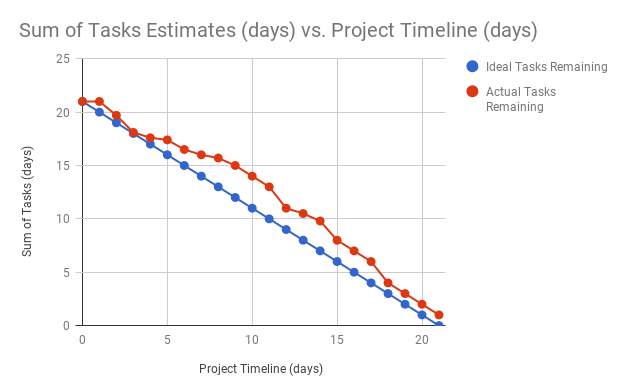
\includegraphics[width=0.6\textwidth]{burndown}
	\caption{A Burndown Chart for the past 14 days.}\label{fig:burn}
\end{figure}

As a team, it was decided that there would only be a single sprint, up until the next point of submission. This was because of the short time period, enough for only a two week sprint. In addition to this, the sprint assessment process was completed more often to ensure that as a team time was managed well and sufficient progress was being made. All the tasks that was set for this sprint were completed within the required time frame.
\subsection{Scrum board}
Again, the scrum board was used to outline and track the completion of each task. The same whiteboard in the John Honey main computer lab was used in order to maintain consistency. This gave a clear visual representation of the objectives. During the sprint, the main jobs required for completion were to further enhance the testing unit to increase its coverage across the implemented systems, implement a simple file converter and introduce a logging system for the server. Much experience was gained from completing previous sprints and so using this experience we were better equipped to handle larger tasks. Examples of the board in use can be found in Appendix \ref{app:board}.

\subsection{Meetings}
Regular meetings were also held to discuss and evaluate progress. This was crucial in the scrum process and as working in a team to allow a point of communication between each member at the same point in time. An example of a major decision being made during the discussion was the change of language of the file converter implementation. It was decided that the more appropriate language to use would be C as there would more extensive libraries for this particular operation and would also have the advantage of greater efficiency. Multiple meetings were held during the most recent sprint to determine the tasks required for completion, to evaluate whether each task was completed and track progress in between.
The minutes for formal meetings are available in Appendix \ref{app:meet}.
